\documentclass[pdflatex,iicol,sn-mathphys-num]{sn-jnl}
\usepackage{graphicx}
\usepackage{amsmath,amssymb}
\usepackage{booktabs}
\usepackage{array}
\usepackage{microtype}
\usepackage{placeins}
\usepackage{seqsplit}
\hypersetup{bookmarksdepth=2}
\raggedbottom
\newcommand{\mae}{\operatorname{MAE}}
\newcommand{\E}{\mathbb{E}}
\begin{document}
\title[Source retention for EV forecasting]{When Does Source Retention Help? A Prequential Study of Low-History EV Charging Demand Forecasting}
\author{AIP491\_G10 Research Team}
\abstract{Models pretrained on established charging stations may improve forecasts at a station with little historical data. How strongly the target model should remain tied to its source representation during online learning is less clear. We evaluate a GRU forecaster whose retention weight is selected from three candidates using paired prediction errors and a bootstrap lower bound on improvement. The evaluation uses 90 selected entities from UrbanEV and six CHARGED city groups, 7/14/28 days of initial target history, three seeds, 14 methods and a 90-day replay. Adaptive has lower station-macro MAE than target-only training in 18 of 21 city--history comparisons, but lower MAE than fixed retention in nine. Against fixed retention, the favorable differences are 1.31--2.36\% in Melbourne, 2.41--2.85\% in S\~ao Paulo and 1.30--1.71\% in CHARGED/Shenzhen. All 18 finite exploratory intervals for this contrast contain zero; the three UrbanEV intervals are undefined. Station-level analysis further shows that individual sites account for most of the Melbourne and S\~ao Paulo reductions. The confidence rule produced fewer recorded switches than selection by past mean error, while next-block continuation audits contain both beneficial and adverse switches. These comparisons show why source-informed gains cannot be treated as evidence for confidence-guided retention selection. They also show where favorable aggregate retention results depend on particular stations, seeds and replay phases.}

\keywords{electric vehicle charging, transfer learning, source retention, online forecasting, prequential evaluation, limited target history}
\maketitle

\section{Introduction}\label{sec:intro}
A newly deployed electric vehicle (EV) charging station has little local history from which to learn a forecasting model. Observations from established stations offer a possible starting point. UrbanEV and CHARGED make station-level charging series available across several urban settings \cite{urbanev2025,charged2025}, allowing this use of source knowledge to be evaluated on more than one target setting. We simulate limited-history targets by restricting the initial observations of existing dataset entities; their identifiers do not establish that the stations were newly opened. We study hourly charging-energy forecasts issued as a complete 24-hour vector, using only information available at the forecast origin.

Source and target stations need not have the same demand level or temporal pattern. A pretrained representation can help fit the initial target observations, yet constrain later updates in an unhelpful direction. Standard fine-tuning leaves this tradeoff to initialization and optimization. An explicit retention penalty makes its strength adjustable: a larger weight penalizes displacement from a frozen source encoder more strongly. A smaller weight relaxes that penalty; it does not change the learning rate or guarantee faster or more accurate adaptation. Selecting that weight once on development data and selecting it repeatedly during deployment are different learning procedures.

Online selection faces a further difficulty. The retention setting with the lowest recent error may have benefited from a few atypical days. Requiring stronger evidence before changing settings could reduce such switches, but the decision still concerns an unobserved future block. Source prediction error, disagreement among source models and changes in recent observations are possible selection signals; none directly measures how much a particular target update benefits from the source constraint.

We implement a three-candidate retention selector for a GRU forecaster. Each candidate predicts before its target labels arrive and then updates on the same available examples. At a decision boundary, paired past-block errors determine whether a challenger has a positive bootstrap lower bound on improvement over the active candidate. The selected model and optimizer state continue into the next block. We compare this procedure with a fixed penalty, selection by past mean error, proxy-based rules and training ablations.

The evaluation has three objectives:
\begin{enumerate}
\item Assess the effects of source initialization and continued retention with 7, 14 or 28 days of initial target history, and examine the relationship between proxy signals and retention benefit.
\item Compare the forecasting accuracy of confidence-guided selection, fixed retention and selection by observed mean error.
\item Characterize variation across stations, seeds, histories and observed contexts, together with recorded computational work.
\end{enumerate}

Our evidence comes from a prespecified evaluation on 90 selected entities, with three seeds and a 90-day online replay. Alongside the method comparisons, we examine the stations contributing to aggregate gains and the next-block consequences of individual switches. Source-informed training helps in many evaluated settings, whereas the additional value of adaptive retention depends on the domain and on how the result is aggregated. The study evaluates this particular learning procedure and cohort; it does not estimate performance across all charging stations represented by the source datasets.

\section{Related work}\label{sec:related}
\subsection{Charging-demand forecasting and the role of public data}
UrbanEV describes station-level charging observations in Shenzhen and also provides regional aggregations \cite{urbanev2025}. We use station identifiers in the processed UrbanEV track. CHARGED harmonizes observations from six cities and reports forecasting, transfer and foundation-model experiments \cite{charged2025}. Its harmonized sites and the UrbanEV stations have different measurement and preprocessing histories. We therefore preserve separate dataset--city groups throughout training and reporting, including separate UrbanEV/Shenzhen and CHARGED/Shenzhen results.

Li et al.'s behavior-guided forecasting preprint models long-term charging patterns, recent behavioral changes and delayed feedback \cite{behavior2026}. Their probabilistic 1- and 4-hour forecasting tasks differ from our direct 24-hour energy-vector task. That work motivates accounting for behavioral variation and label timing; it is not a matched numerical baseline for the experiments reported here. Our forecaster uses historical energy, its observation mask and calendar variables, without the additional behavior representation proposed there.

\subsection{Pretrained weights and continuing source constraints}
Transfer learning uses information from a source task or domain to support a target learner \cite{pan2010}. In neural fine-tuning, pretrained weights supply an initial state even when no source penalty appears in the target objective. Li et al. study regularization toward pretrained parameters and recommend an explicit parameter-space reference for their convolutional transfer tasks \cite{li2018}. Our primary constraint compares source and target encoder outputs on the same target history. Source-derived coordinate scales normalize this representation penalty. We evaluate an encoder-parameter penalty separately, using the same candidate-selection procedure; the two penalties have different numerical scales.

R-Tuning combines frequency-aware replay with a latent consistency constraint during continual time-series adaptation \cite{rtuning2026}. Thus retaining prior representations is not, by itself, a new idea. Our experiment uses a fixed source encoder without synthetic source replay and evaluates how its penalty weight is selected.

This distinction determines the comparisons needed in the present study. Target-only training measures a complete procedure without source initialization or retention. Full fine-tuning retains source initialization but removes the continuing penalty. Fixed retention adds a constant constraint, while Adaptive changes its weight during replay. Because those procedures follow different optimization trajectories, their eventual errors cannot be attributed to a single component without considering their initialization and update rules.

\subsection{Online transfer, selection and prequential evaluation}
McKay et al.'s BOTL framework transfers models among online domains and combines their predictions with a local meta-learner \cite{botl2020}. Our source model is instead trained before target deployment and remains frozen. Adaptation occurs within each target model, and selection changes the strength of a representation constraint rather than the ensemble weight of a transferred predictor. This choice isolates a practical setting in which historical source models are available but ongoing source streams are not used.

Hyperon couples stream learning with evolutionary hyperparameter search \cite{hyperon2025}. We study a fixed retention grid, allowing the same candidates and update budget to be used by confidence-guided and mean-only selectors. Their difference is the decision rule applied to paired candidate errors. Once the selectors make different decisions, their retained states can diverge; the comparison therefore measures the complete online procedures.

GUARD routes among foundation-model teachers and gates distillation using uncertainty \cite{guard2026}; PADRE combines delayed-residual and contextual evidence to gate online gradient updates \cite{padre2026}. These are relevant precedents for evidence-dependent adaptation, but our proxy rules are not reproductions of either framework. None of these external systems was rerun under the present 24-hour protocol, so the internal comparisons establish no ranking against them.

Prequential evaluation assesses predictions as an evolving learner encounters new observations \cite{gama2013}. We follow forecast-before-label ordering and apply updates after complete label vectors become available. Block resampling, following the broader approach of dependence-aware bootstrap methods \cite{kunsch1989}, is used for candidate decisions and exploratory method comparisons. The two applications have different resampling units, described below. Short streams, missing dates and changes in the data distribution restrict the interpretation of their uncertainty estimates.

\section{Forecasting and retention method}\label{sec:method}
\subsection{Task, scale and available information}
For target station $i$, at daily origin $t$ we forecast the next 24 hourly charging-energy values $y_{i,t,h}$, $h=0,\ldots,23$, from the preceding 24 hours and known calendar variables. A single model evaluation produces all 24 outputs. Initial target history is $H\in\{7,14,28\}$ days before deployment. After deployment, complete newly available target observations continue to support online updates.

Each historical hour has seven features: scaled energy, sine and cosine of hour, sine and cosine of weekday, a weekend indicator and an energy-present mask. Five calendar features are supplied for each future hour. No future weather, price or observed target energy is supplied. Energy is divided by a station-specific 95th percentile fitted on valid available predeployment observations; a nonpositive percentile uses a declared 1 kWh scale. The fitted scale is held fixed during replay. Missing historical energy is encoded as zero in the energy feature and zero in the observation mask, distinguishing it from an observed zero with mask one. Target labels remain missing: a daily label vector is trainable and scoreable only when all 24 valid values are available.

\subsection{GRU forecaster and objective}
The encoder is a two-layer GRU with hidden dimension 64 and zero dropout, using the GRU family introduced by Cho et al. \cite{cho2014}. Its final top-layer hidden state $z_\theta(X)\in\mathbb{R}^{64}$ is concatenated with the 120 future-calendar values. The forecasting head is a linear layer of width 64, a ReLU and a linear map to 24 outputs followed by Softplus. Thus predicted normalized demand is nonnegative. All target-network parameters remain trainable.

Let $\theta_S$ denote the fixed source model. For one daily example the training objective is
{\interdisplaylinepenalty=10000
\begin{align}
 \mathcal L(\theta;\lambda)&=\frac{1}{24}\sum_{h=0}^{23}|\widehat{\widetilde y}_{\theta,h}-\widetilde y_h|+\lambda\mathcal R(\theta,\theta_S),\label{eq:loss}\\
 \mathcal R(\theta,\theta_S)&=\frac{1}{64}\sum_{j=1}^{64}\left(\frac{z_{\theta,j}(X)-z_{\theta_S,j}(X)}{\sigma_{S,j}+\epsilon}\right)^2.\label{eq:retention}
\end{align}
}
Here $\widetilde y=y/s_i$, $s_i$ is the target energy scale, $\sigma_{S,j}$ is the population standard deviation of source latent coordinate $j$ over source training examples, and $\epsilon=10^{-3}$. The source outputs and latent scales are fixed during target training and detached from its gradients. The coefficient $\lambda$ controls the loss penalty. At $\lambda=0$, the target keeps its existing weights and optimizer state, including the effects of source initialization and earlier updates.

There is one source checkpoint per namespace and seed, reused across target stations and histories within that namespace: 21 checkpoints in total. Sources are trained for 10 epochs. Both encoder and compatible head weights are copied from Source. Initial target adaptation uses three epochs and a fresh Adam optimizer when complete prefix training examples exist; otherwise this stage is skipped and the source-initialized or random target state is retained, according to the method. Online adaptation uses one epoch per newly available complete daily example. Batch size is 64 and learning rate is $10^{-3}$. A single online daily record therefore requires one optimizer step per candidate. Source optimizer state is not transferred initially. These settings are fixed for the reported Final evaluation.

\subsection{Confidence-guided candidate selection}
Adaptive uses $\Lambda=\{0,0.1,1\}$, starts at $\lambda_a=0.1$, and has 14-day decision blocks. At a block's start, all candidate branches are cloned from the selected trained state, including model weights, Adam state and recorded random state. Each candidate issues its forecast before observing the corresponding labels, and each receives the same newly available training examples under its own retention weight. Only the active branch supplies the deployed forecast. At a boundary, the selected candidate's \emph{trained} state is carried forward and reforked; candidates are not reset to the beginning of the previous block.

For valid day $d$ in the completed block, let $\ell_{a,d}$ and $\ell_{c,d}$ be normalized daily MAE of active and challenger branches. Define paired improvement
\begin{equation}
 \begin{aligned}d_{c,d}&=\ell_{a,d}-\ell_{c,d},\\L_c&=Q_{\alpha/2}\!\left(\overline d_c^{*(1)},\ldots,\overline d_c^{*(2000)}\right).\end{aligned}\label{eq:lcb}
\end{equation}
The two challengers share bootstrap day indices. The controller samples noncircular overlapping three-observation segments from the chronological valid-day sequence, concatenating and trimming to the original sequence length. Quantiles use linear interpolation. With $\alpha=0.05$, the lower quantile is 0.025 for each challenger (a two-challenger adjustment). A candidate qualifies when $L_c>\delta$, where the locked margin is $\delta=0$. The qualifying candidate with the largest bound is selected, breaking ties by proximity to the active weight and then the fixed grid order. If no candidate qualifies, or fewer than seven valid daily vectors exist, the active trained branch is retained. Boundary timestamps and label availability are checked explicitly.

The decision statistic estimates improvement within the completed block. We assess its relationship to subsequent error using the continuation audits in Section~\ref{sec:switch}. Missing calendar dates are compressed into valid-observation order in the \emph{controller} bootstrap, so an ordinal segment can cross a calendar gap. This differs from the final-comparison bootstrap in Section~\ref{sec:metrics}, which preserves scheduled calendar dates. Repeated testing, short blocks and temporal changes further restrict a formal confidence interpretation.

\begin{figure*}[t]\centering
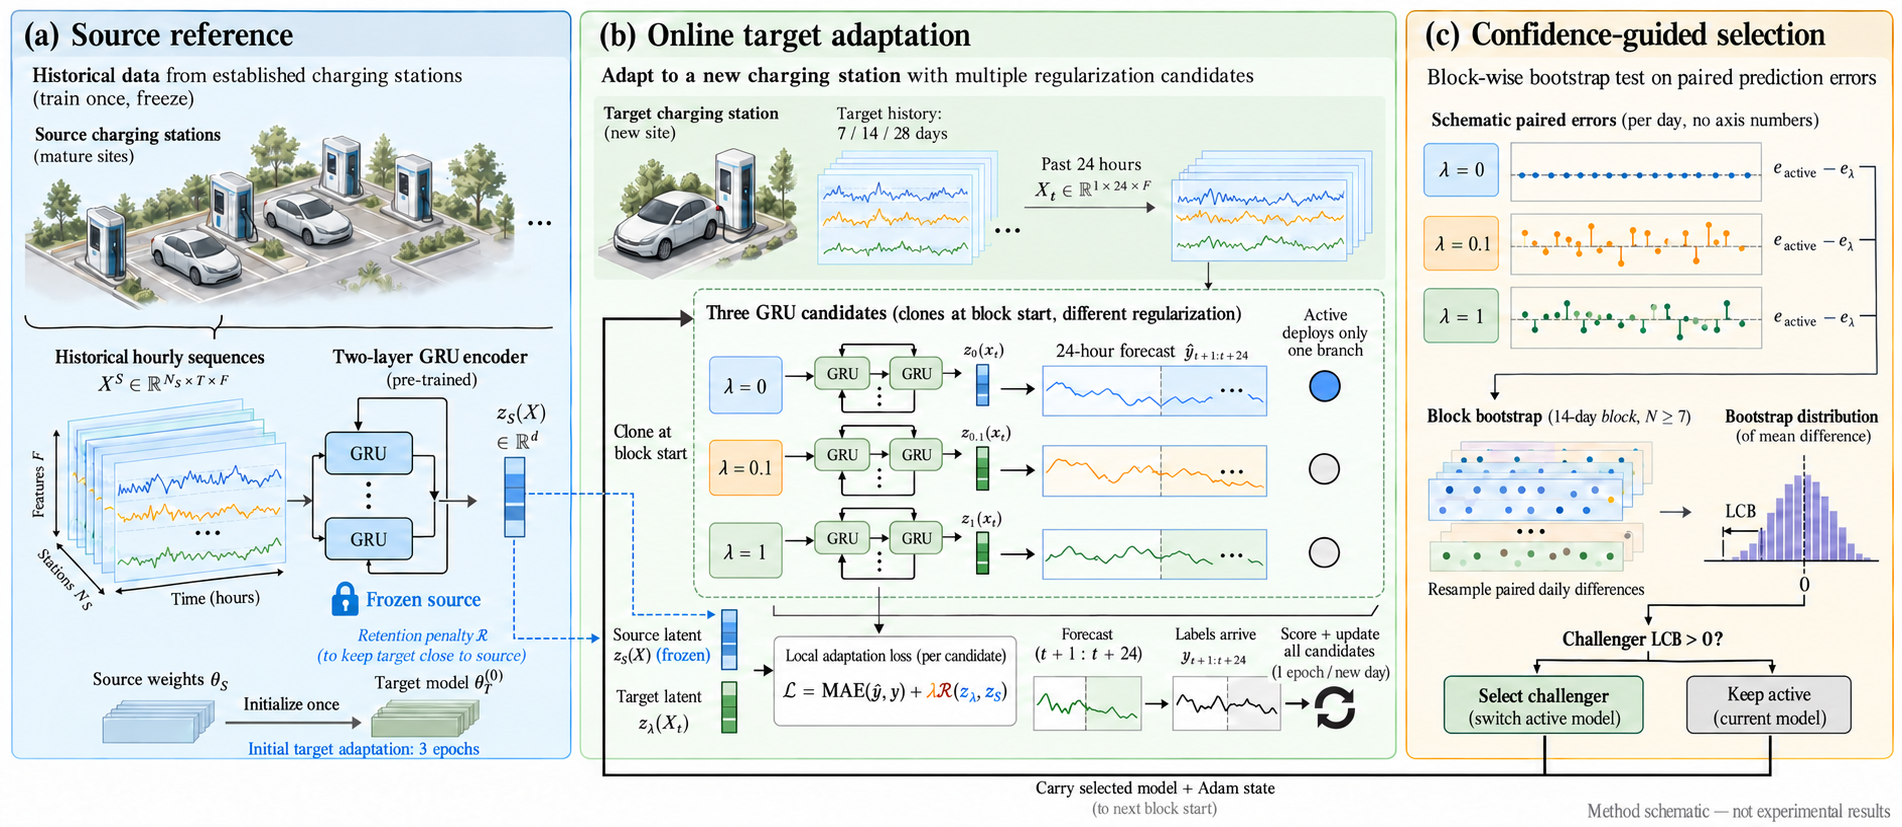
\includegraphics[width=\textwidth]{fig-protocol-illustrated-v5.png}
\caption{Illustrated retention procedure shared by UrbanEV/SZH and all six CHARGED city groups. Source and target remain within the same dataset/city group in each experiment. The source encoder and latent scales remain frozen during target learning. Initial target adaptation uses three epochs; online updates use one epoch per newly available complete daily vector. At each 14-day block start, three candidates clone the selected model and Adam state. Only the active forecast is deployed. Paired completed-block errors determine whether a challenger qualifies; otherwise the active trained state is retained. The blue branch illustrates an active $\lambda=0$ after a possible switch, not the initial $\lambda=0.1$. The initial three-epoch adaptation is conditional on complete prefix examples. The drawn GRU branches abbreviate the full forecaster: the future-calendar input, MLP/Softplus head, mask and scaling operations are specified in the text. Internal GRU drawings are icons, not literal layer/gate wiring. Signals, errors and bootstrap shapes are schematic, not experimental results; the loss and resampling rule are defined in the text.}\label{fig:protocol}
\end{figure*}

\subsection{Comparators and ablations}\label{sec:comparators}
Fourteen distinct methods are evaluated. Online-best shares Adaptive's three candidates, initial weight, update schedule and minimum evidence rule, but chooses the lowest observed mean error. Since $\delta=0$, a separate mean-only ``without confidence'' label would duplicate this definition and is not counted as a fifteenth method. Fixed uses $\lambda=1$ from initial adaptation onward, whereas Adaptive and Online-best start at 0.1. The Adaptive--Fixed contrast includes this initial-penalty difference. Online-best provides the closer comparison for the confidence decision rule because its initialization and candidate training agree with Adaptive.

Proxy rules use the mean available block signal and two locked thresholds. Source error is normalized frozen-source MAE with thresholds (0.1, 0.5). Uncertainty is mean horizon-wise population standard deviation of the three frozen source-seed forecasts, with thresholds (0.01, 0.05). Drift is the root-mean-square standardized change in historical mean, maximum and zero proportion from prefix descriptor moments, with thresholds (1, 3). Increasing signal bins map to weights (1, 0.1, 0); insufficient available evidence preserves the active weight. The mappings are prespecified selection rules; their signal values are not calibrated probabilities.

\paragraph{Reference forecasts.} Frozen Source predicts without target training. Seasonal naive uses an available weekly lag, falling back to the daily lag, the available-history mean and then zero. Target-only trains from random weights; Full fine-tuning starts from Source and uses no continuing penalty.
\paragraph{Ablations.} Parameter retention replaces the representation penalty with mean squared displacement of encoder parameters from Source, excluding the prediction head. No Source initialization starts from random target weights but keeps the frozen source representation reference. The 7- and 28-day block variants change the Adaptive decision interval. The complete 14-method comparison is visualized in Supplement S1, with exact MAE and RMSE in the accompanying CSV.


\section{Experimental design}\label{sec:experiment}
\subsection{Datasets and selected cohorts}
Figure labels use dataset/city identifiers: AMS (Amsterdam), JHB (Johannesburg), LOA (Los Angeles), MEL (Melbourne), SPO (S\~ao Paulo) and SZH (Shenzhen). UrbanEV/SZH and CHARGED/SZH are separate namespaces. The former uses the UrbanEV release, and the latter uses CHARGED's Shenzhen series. They are not pooled and do not constitute two independent geographic replications. UrbanEV observations cover September 2022 to February 2023 in this processing track; deployment is 1 December 2022. CHARGED covers April--September 2023; deployment is 1 July 2023. The scheduled replay length is 90 days in both tracks. The task predicts the released/processed hourly charging-energy series in kWh, rather than directly metered latent demand free of publisher estimation or preprocessing assumptions.

Entity identifiers are assigned to Source, Development and Final by a fixed salted SHA256 threshold rule with approximate 60/20/20 proportions. This separates identifiers; physically colocated identifiers may remain in different partitions. Development determines the source-epoch, retention, controller and proxy configurations before the frozen Final run. Final selection is a deterministic, outcome-blind bounded subset of eligible identifiers, with 30 UrbanEV IDs and 10 IDs in each CHARGED city. Sampling is bounded by the available execution budget, so its results describe the selected cohort. Table~\ref{tab:scope} summarizes the scored scope; Supplement S1 records the inventory and eligibility denominators. UrbanEV readiness differs slightly by initial-history budget; a station--budget pair is not a distinct station.

\begin{table}[t]\centering\small
\caption{Primary target cohorts. The exact eligible pools and released inventories are retained in the supporting data description.}\label{tab:scope}
\begin{tabular}{@{}lrr@{}}\toprule
Group & N / scored & Raw (\%)\\\midrule
UrbanEV/SZH & 30 / 29 & 1.78\\
CHARGED/AMS & 10 / 10 & 0.41\\
CHARGED/JHB & 10 / 10 & 21.28\\
CHARGED/LOA & 10 / 10 & 4.37\\
CHARGED/MEL & 10 / 10 & 15.87\\
CHARGED/SPO & 10 / 10 & 21.28\\
CHARGED/SZH & 10 / 10 & 0.69\\\botrule
\end{tabular}\end{table}


The CHARGED total is 60 selected IDs out of 4,280 (1.40\%). Its site inventory is a harmonized/virtual-site representation and should not be equated directly with a uniform count of physical chargers. SPO includes all ten metadata-ready Final IDs, but this is only a census of that eligible partition. The primary Final has 270 entity--history pairs and seeds 42, 43 and 44, giving 810 whole units and 11,340 method--seed cells. UrbanEV station 2193 has no scoreable replay outcome and remains declared. Its $3\times3\times14=126$ cells are null, leaving 11,214 scored cells and 89 scored entities. 

\subsection{Temporal protocol and frozen settings}
The pipeline separates forecast issue time, label availability and update time. Historical input masks distinguish absent/unavailable observations from valid zeros. A forecast cannot use its own labels, and a partially observed 24-hour vector is not scored or trained. Later label arrival does not retroactively change the issued forecast. Sources are trained only on their permitted predeployment inputs; each namespace reuses its own source checkpoints without cross-city weight pooling.

The selected source epoch is 10; retention candidates are 0, 0.1 and 1; Fixed is 1; the principal block size is 14; and the controller uses seven minimum valid days, 2,000 resamples and a zero improvement margin. The configuration selected during Development is held fixed for Final. Calibration used the bounded UrbanEV Development cohort and staged finite searches: Source durations of 1, 3 and 10 epochs; four positive Fixed weights from 0.001 to 1; and four joint recipes each for the controller and proxy/parameter rules. These searches do not isolate individual hyperparameter effects or establish equal tuning compute. The selected Source duration and Fixed weight lie at their search endpoints. Alpha and resample count were held fixed during controller calibration, not exhaustively optimized. The selected recipe is shared across cities rather than optimized separately on their Final outcomes.

Availability is enforced under recorded replay assumptions. CHARGED uses publisher-local naive clocks; the original collection/arrival process and daylight-saving-time treatment are not independently established by these checks. Publisher harmonization or imputation may already affect released series. UrbanEV's mask-preserving processing and local causality checks do not establish causal availability of every upstream source. These limits apply to deployment interpretation even when the local replay is temporally consistent.

\subsection{Metrics, aggregation and uncertainty}\label{sec:metrics}
For method $m$, station $i$, seed $s$ and its valid daily origins $D_i$, daily MAE is the mean absolute error over the 24 hourly values in original kWh. We first average origins and paired seeds within station, then average stations equally within each namespace and history:
\begin{equation}
 \begin{aligned}e_{m,i,s,d}&=\frac{1}{24}\sum_{h=0}^{23}|\widehat y_{m,i,s,d,h}-y_{i,d,h}|,\\ M_m&=\frac{1}{N}\sum_{i=1}^N\frac{1}{3}\sum_{s}\frac{1}{|D_i|}\sum_{d\in D_i}e_{m,i,s,d}.\end{aligned}\label{eq:macro}
\end{equation}
Method pairs use matched scoreable origins. RMSE is computed within the recorded station--seed evaluation and macro-averaged in the same station-first manner; it is not the square root of a city-pooled squared error. The principal contrast is $\Delta_{A,C}=M_A-M_C$, and its relative version is $100\Delta_{A,C}/M_C$. Negative contrasts favor Adaptive. We do not average absolute kWh across cities or treat seeds, days and repeated history panels as independent stations.

For station-level transfer gain, we compare three-seed mean MAEs against Target-only: $g_i=(\overline e_{T,i}-\overline e_{m,i})/\overline e_{T,i}$ when $\overline e_{T,i}>0$. The negative-transfer rate is the fraction of stations with $g_i<0$ among those with positive baseline MAE, not a fraction of days or seed runs. Zero-baseline cases retain an absolute difference and an undefined gain. The CSV reports the denominator. Any negative sign counts, so NTR is not a practical-harm or significance threshold.

Frozen exploratory 95\% intervals resample paired stations and circular seven-day calendar blocks over the common 90-day schedule, using 2,000 replicates, seed 20261026 and the fixed three-seed average. The same calendar indices are used across sampled stations. Missing dates remain missing. If any sampled station mean is undefined in any replicate, the interval remains null rather than dropping undefined replicates. UrbanEV has 40 undefined replicates in each reported comparison, so its intervals are null. The intervals are conditional on small selected cohorts, with possible colocation, circular seams, nonstationarity and no simultaneous-comparison correction. Inclusion of zero is neither evidence of equivalence nor proof of no effect.

\subsection{Post hoc diagnostics and evidence verification}
The completed Final summaries already define weekday/weekend, replay phases (days 1--30, 31--60 and 61--90), and sparse/dense prefix contexts using Development-frozen thresholds. We additionally summarize station direction counts, leave-one-station-out (LOO) gaps and per-seed contrasts. These are post hoc descriptive analyses, not new confirmatory tests or a basis for selecting favorable stations. LOO recomputes the mean after each possible single omission; every full-cohort result remains primary.

All seven summaries, seven run tables, seven derived metadata files and seven daily-error CSVs were checked against their recorded SHA256 identities. We reconciled 942,102 scored daily method rows with all 11,214 scored cell means and counts, retaining the 126 null cells. The maximum per-cell MAE arithmetic discrepancy was $4.55\times10^{-13}$ kWh. The post hoc analysis uses these recorded errors and summaries; model fits, selected hyperparameters and original bootstrap outputs are unchanged.

\section{Results}\label{sec:results}
\subsection{Source-informed learning across the evaluated domains}\label{sec:transfer}

Figure~\ref{fig:comparisons} gives the principal selector contrasts. Supplement S1 visualizes all 14 methods, and the accompanying CSV contains exact MAE/RMSE for every group and history. Adaptive has lower macro MAE than Target-only in 18 panels, while all three AMS panels are adverse. Among the frozen finite intervals against Target-only, 15 favor Adaptive and three favor Target-only; three UrbanEV intervals are undefined. This is evidence for useful source-informed learning in many evaluated settings, not for the confidence gate specifically. Adaptive differs from Target-only in initialization, retention, candidate selection and computational work.

UrbanEV illustrates the distinction. Adaptive MAE is 8.1014, 8.0517 and 8.0015 kWh for 7, 14 and 28 days, versus Target-only 13.4341, 13.4132 and 13.3079 kWh. Yet Fixed is better than Adaptive at every history. Thus a substantial transfer gain coexists with an unfavorable Adaptive--Fixed contrast. LOA similarly shows useful transfer but small, mixed selector differences.

In JHB, Frozen Source has the lowest point MAE among all 14 methods, 0.9623, 0.9645 and 0.8670 kWh, versus Adaptive 1.3685, 1.3604 and 1.3560. Target updates can degrade a useful pretrained model under the evaluated recipe. Conversely, in CHARGED/SZH, Full fine-tuning is lower than Adaptive at every history (88.8440/88.5427/88.1054 versus 90.6306/89.3300/89.3310 kWh). Source initialization followed by unconstrained adaptation is therefore a stronger point-MAE alternative there. Seasonal naive is the lowest-MAE method in that namespace, although it has worse RMSE than Adaptive. The MAE and RMSE rankings consequently differ for these two methods.

AMS is the strongest adverse domain. Adaptive is approximately 132.5--140.9\% worse than Target-only, and Seasonal naive is much better than either in macro MAE. Its station-level NTR is 5/10 at every history; the adverse macro difference does not mean that every AMS site experiences negative transfer. At seven days, the three Adaptive seed means are 8.9838, 0.5001 and 8.9838 kWh; Target-only gives 2.6729, 2.6409 and 2.3724. Fixed and Full fine-tuning also show the adverse source-informed aggregate pattern. The same seeds control several random components, so these data do not isolate source quality as a cause. Aggregate scores alone also do not diagnose a particular prediction collapse. They do show that changing the continuing penalty is not demonstrated to repair every source-related failure.

\subsection{Adaptive versus fixed and mean-only online selection}\label{sec:selection}
\begin{figure*}[t]\centering
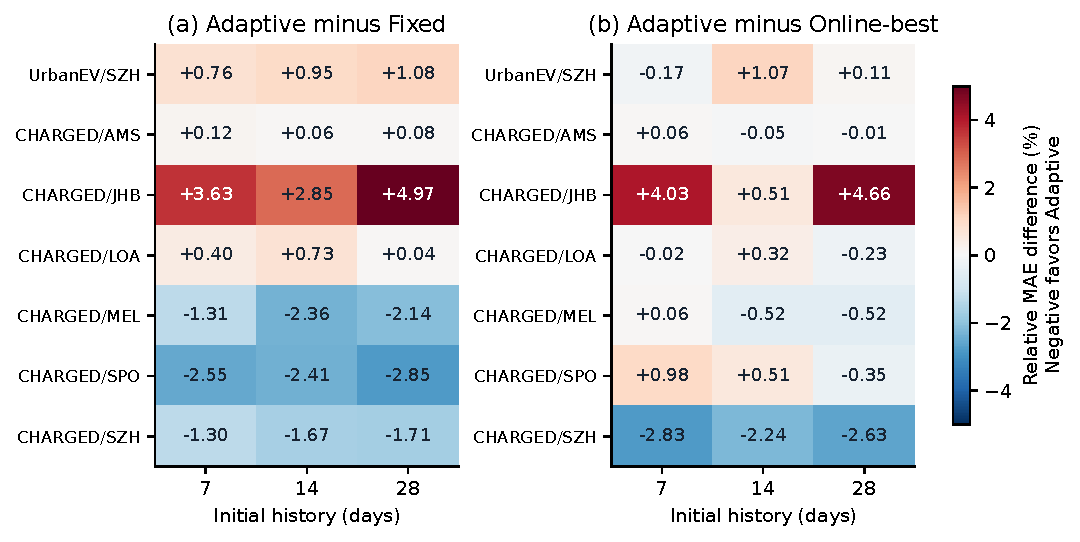
\includegraphics[width=\textwidth]{fig-comparisons-v8.pdf}
\caption{Relative MAE contrasts for UrbanEV/SZH and the six CHARGED city groups. Negative values favor Adaptive. Colors share a $\pm5\%$ scale; values are printed explicitly. Favorable point estimates are not significance claims: all 18 finite intervals in each comparison include zero, and the three UrbanEV intervals are undefined.}\label{fig:comparisons}
\end{figure*}
Adaptive improves on Fixed in 9 of 21 panels and is worse in 12 (Figure~\ref{fig:comparisons}). All favorable macro directions occur in MEL, SPO and CHARGED/SZH, at all three histories. MEL reductions are 1.31\%, 2.36\% and 2.14\%; SPO reductions are 2.55\%, 2.41\% and 2.85\%; and CHARGED/SZH reductions are 1.30\%, 1.67\% and 1.71\%. At the other extreme, JHB increases are 3.63\%, 2.85\% and 4.97\%. UrbanEV is worse by 0.76--1.08\%; AMS and LOA have smaller unfavorable macro gaps.

Against Online-best, Adaptive is lower in 11 panels and higher in 10. CHARGED/SZH has favorable contrasts at all histories (2.24--2.83\% lower); SPO favors Online-best at 7 and 14 days. Adaptive has the lowest point MAE among all 14 methods only in SPO at 28 days. The 7- and 28-day block variants are stronger MEL alternatives, showing that confidence is not the only relevant design choice.

All 18 finite Adaptive--Fixed intervals and all 18 finite Adaptive--Online-best intervals include zero (Supplement S1). For example, MEL/14 has an Adaptive--Fixed gap of $-1.2815$ kWh with interval $[-6.0458,0.1916]$. The uncertainty in these estimates permits both favorable and adverse Adaptive effects. Adaptive is also lower than Full fine-tuning in 17 panels, with six finite intervals below zero, twelve crossing zero and three undefined. This supports studying retention-based learning, but the contrast does not isolate confidence from the retained learning trajectory or other design choices.

\subsection{Station contributions to favorable macro differences}\label{sec:concentration}
\begin{figure*}[t]\centering
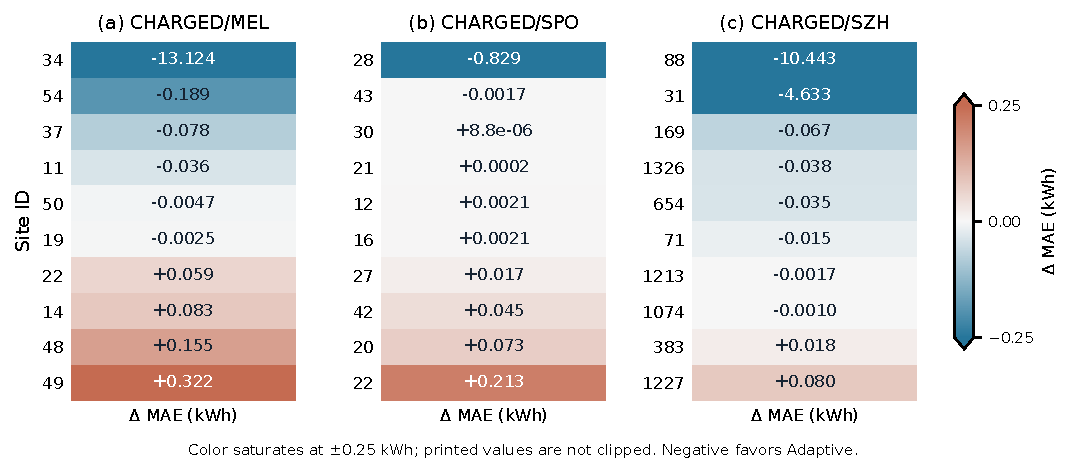
\includegraphics[width=\textwidth]{fig-station-gaps-heatmap-v8.pdf}
\caption{Station-level Adaptive--Fixed MAE gaps (kWh) at 14-day initial history in CHARGED/MEL, CHARGED/SPO and CHARGED/SZH, the three groups with favorable macro contrasts. Values average the three paired seeds; negative favors Adaptive. Sites are sorted separately within each group, so rows do not identify matched sites across cities. All panels share a color scale saturated at $\pm0.25$ kWh; the printed values retain their actual magnitudes. All ten sites per group remain included. Large absolute-error contrasts can dominate the macro gap; this does not establish that the corresponding physical stations are larger.}\label{fig:stations}
\end{figure*}
Figure~\ref{fig:stations} shows the station-level terms underlying the three favorable macro comparisons. MEL has lower Adaptive MAE at 6/10 stations at every history. However, site 34 contributes approximately 103\%, 102\% and 89\% of the signed net reduction. A contribution above 100\% means that other sites partly offset its gain. Removing that site reverses the mean at 7 and 14 days, to $+0.0224$ and $+0.0344$ kWh. At 28 days every single-omission mean remains favorable, with the weakest gap $-0.1424$ kWh. Seed 42 favors Fixed at 14 and 28 days despite the favorable three-seed mean.

SPO has lower Adaptive MAE at only 4/10, 2/10 and 3/10 stations. Site 28 accounts for about 188\%, 173\% and 133\% of the net reduction. Omitting it reverses the mean at every history ($+0.0501$, $+0.0389$, $+0.0213$ kWh), and the median station gap favors Fixed at every history. Nevertheless, each seed's namespace average favors Adaptive. Seed consistency therefore does not establish broad station-level benefit.

CHARGED/SZH is less fragile to one omission: every LOO mean remains favorable at every history, with the weakest gaps $-0.4316$, $-0.5214$ and $-0.5658$ kWh. Site 88 still contributes about 67--69\% of the net reduction, and seed 42 favors Fixed at every history. Adaptive improves on Fixed at 6/10, 8/10 and 3/10 sites; its median gap is unfavorable at 28 days. Thus the mean direction is less dependent on a single selected site than in MEL or SPO, while the seed sensitivity and stronger alternative baselines remain.

\subsection{Initial-history and replay-phase differences}
\begin{figure*}[t]\centering
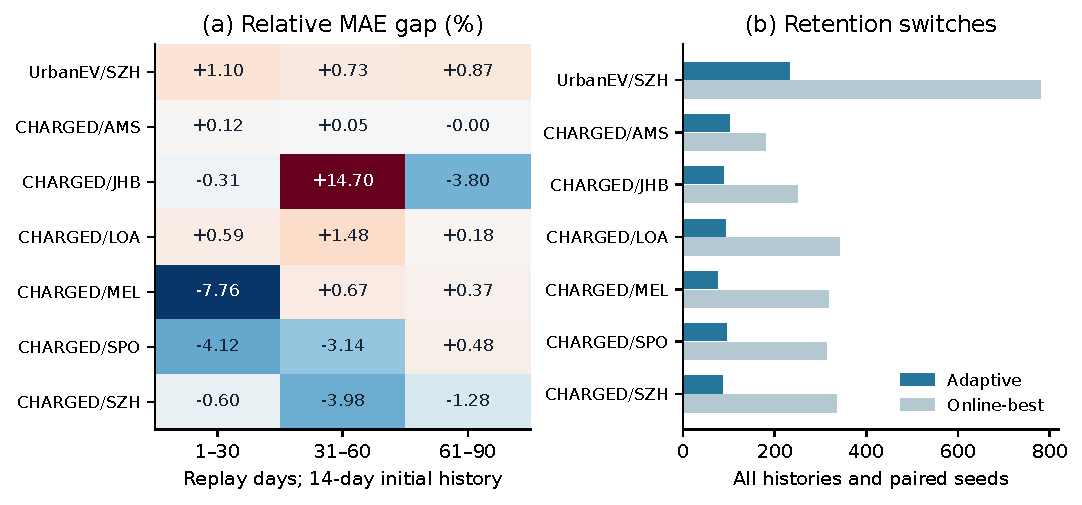
\includegraphics[width=\textwidth]{fig-phase-switching-v8.pdf}
\caption{(a) Adaptive--Fixed relative MAE gaps by replay phase at 14-day initial history. Negative favors Adaptive. The JHB middle-phase value exceeds the shared color range and is printed in full. (b) Retention-switch counts over all histories and seeds. Fewer switches describe policy behavior, not better accuracy or lower total computation.}\label{fig:phase}
\end{figure*}
Increasing initial history does not monotonically improve every method or guarantee an Adaptive advantage. In MEL, for example, Adaptive's absolute MAE increases from 52.1542 at seven days to 53.0840 at 14 days, while remaining lower than Fixed. A history comparison changes the predeployment training examples and scale, so it is not an isolated causal estimate of the value of one extra day of data.

At 14-day initial history, MEL's relative Adaptive--Fixed contrasts over successive 30-day phases are $-7.76\%$, $+0.67\%$ and $+0.37\%$ (Figure~\ref{fig:phase}). Its full-stream gain is chiefly early, rather than sustained improvement throughout deployment. SPO is favorable in the first two phases and slightly adverse in the last ($-4.12\%$, $-3.14\%$, $+0.48\%$); SPO/28 is favorable in all three phases, but the station concentration remains. JHB changes sign ($-0.31\%$, $+14.70\%$, $-3.80\%$). These patterns do not identify a prospectively reliable switching time.

Prefix contexts also differ. At 14 days, MEL favors Adaptive in the six dense-prefix sites ($-2.58\%$) but not the four sparse-prefix sites ($+0.99\%$); SPO favors it in the four sparse sites ($-3.05\%$), not the six dense sites ($+3.15\%$). These thresholds were frozen on Development, but the subgroup interpretations are descriptive and confounded by which stations comprise each group. We do not construct a new context-specific controller from Final outcomes.

\subsection{Switching decisions and subsequent prediction error}\label{sec:switch}
Across all histories and seeds, Adaptive makes 232, 101, 89, 92, 75, 94 and 86 switches in UrbanEV, AMS, JHB, LOA, MEL, SPO and CHARGED/SZH, respectively. Online-best makes 780, 180, 250, 341, 317, 313 and 335. Adaptive switches less in every namespace and at every history. UrbanEV records 315 insufficient-evidence boundaries. Both upward and downward changes occur, so the policy acts as a bidirectional selector rather than a retention-decay schedule.

At selected switch checkpoints, the evaluation also continues the previous policy through the next block. This provides a paired new-minus-old error contrast from the switch state. The results are mixed. MEL/14 has a median contrast of $+0.1007$ kWh, favoring the old policy. CHARGED/SZH has positive median contrasts at all three histories despite its favorable full-path Adaptive--Fixed means. In AMS, many negative audit signs have median magnitudes around $10^{-11}$ kWh and therefore convey little about practical improvement. Supplement S1 reports the audit coverage and exact-sign counts. These local continuation comparisons explain why a reduction in switching cannot by itself establish better future forecasting. Unlike the planned practical-harm rate, the frozen audit profile supplies no locked minimum-harm threshold; exact signs cannot be relabeled as that rate. No recovery time is reported because no independently defined change event and recovery criterion were evaluated.

\subsection{Proxy relationships and computational work}
The saved proxy analysis correlates signals with same-block candidate benefit (zero-retention minus high-retention MAE) on each proxy controller's own path. At 14 days, mean defined-station Pearson correlations for source error range from $-0.322$ to $+0.030$, uncertainty from $-0.217$ to $+0.519$, and drift from $-0.161$ to $+0.068$. Defined coverage ranges from 5/10 to 9/10 CHARGED sites and 27/30 UrbanEV sites; constant or incomplete cases remain undefined. These short-series correlations are not next-block predictive validation or a shared-path causal comparison of proxies. They reinforce the distinction between a signal and relative retention benefit, without proving that the confidence selector solves the latter problem.

Recorded main candidate-update counts are exactly three times Fixed: 24,300 versus 8,100 per CHARGED namespace and 56,079 versus 18,693 for UrbanEV, over all histories and seeds. Adaptive and Online-best have equal main candidate-step counts. Adaptive has fewer recorded continuation-audit steps because it switches less, but those branches are evaluation overhead, not information available to the deployed controller. Source pretraining, initial adaptation, setup, restoration and export are separate costs. These counters establish extra update work relative to Fixed; they are not complete wall-time, FLOP, energy or billable-GPU ratios.

A separate three-station implementation is reported in Supplement S1. It uses different source states, seeds and model/controller details and is excluded from the primary averages.

\section{Discussion}\label{sec:discussion}
\subsection{Source initialization and later adaptation serve different roles}
The evaluated domains require different interpretations of source knowledge. In UrbanEV, the large Adaptive--Target-only difference coexists with lower error from Fixed at every history. Much of the practical benefit can therefore be obtained by a simpler source-informed method. JHB goes further: the frozen model is better than every tested adaptation procedure in point MAE. In CHARGED/SZH, source-initialized fine-tuning is better than Adaptive at every history, although Adaptive improves on Fixed and Online-best. These observations support examining the starting model and the later constraint separately. Here source usefulness is operationalized through forecast-error contrasts between specified learning procedures, not a measured quantity of stored knowledge. We did not re-evaluate forgetting on source stations after target adaptation.

AMS exposes a limitation of the available intervention. Adaptive can select zero retention, but it cannot return to a random initialization or an earlier trajectory. Poor forecasts inherited from source initialization or from subsequent optimization need not be repaired by reducing the current penalty. The adverse source-informed AMS results are consistent with this limitation. Their cause cannot be assigned to initialization alone because source training, target updates and several random components vary with the same seed.

\subsection{What confidence changes in this experiment}
The confidence rule changes decisions: compared with Online-best it produces fewer switches at every history in every city group. Both procedures train the same number of main candidate updates, so this difference follows from selection rather than a smaller candidate budget. Its accuracy consequences are less consistent. Past-block lower bounds can favor a challenger whose next-block advantage disappears, while an incumbent can remain active when seven valid days are unavailable. The continuation audits document both beneficial and adverse outcomes after switches.

The favorable MEL and SPO means also show why seed averages are insufficient to characterize the benefit. SPO favors Adaptive under each seed, yet omitting one site reverses the macro direction at every history. MEL's largest gain occurs in the first 30 replay days; later phases favor Fixed at the 14-day history. A controller evaluated only by the final average would conceal these dependencies. CHARGED/SZH retains a favorable macro direction under every single-site omission, but its seed sensitivity and lower errors from Full fine-tuning and Seasonal naive still affect the choice of forecasting procedure.

The present results therefore support a specific behavioral finding---more conservative retention selection---and localized accuracy differences. The ability of boundary-available evidence to predict a new retention setting's benefit in the following block remains unresolved. Same-block proxy correlations and retrospective phase descriptions do not establish that predictive ability. They identify limitations to address in a subsequent study with new evaluation data.

\subsection{Limitations}
\paragraph{Evaluation scope.}
The findings characterize source retention within the selected cohorts; they do not validate a prospective rule for unseen stations or a general accuracy benefit from confidence. Proxy correlations, context summaries and continuation audits are exploratory. The evaluation does not include complete end-to-end runtime/memory comparisons or thresholded practical-harm rates. Archived-output checks do not constitute independent checkpoint reproduction.

\paragraph{Cohort and measurements.}
The selected cohorts are deterministic and small relative to several city inventories. They do not support population-level accuracy estimates. Identifier partitions may contain colocated infrastructure; UrbanEV/Shenzhen and CHARGED/Shenzhen share a city and are evaluated as separate data products rather than independent geographic replications. The target is released hourly charging energy. Publisher estimation, harmonization and imputation can affect the measured quantity before our processing begins. Recorded replay timing also depends on arrival assumptions and publisher-local clocks, including unresolved daylight-saving-time behavior in CHARGED.

\paragraph{Learning procedures.}
The experiments use one GRU architecture, a three-weight grid, a shared development-selected configuration and three seeds. Fixed and Adaptive differ in their initial penalties. Parameter-space and representation-space penalties have different scales, and the proxy methods use fixed threshold mappings. Thus the rankings concern the implemented procedures under their stated training budgets. External forecasting architectures and foundation models were not rerun under this protocol. The three-candidate procedures also require more main update steps than Fixed; recorded counters do not establish complete end-to-end runtime or resource consumption.

\paragraph{Statistical interpretation.}
The three history panels share entities and source checkpoints, and seeds are averaged within stations rather than treated as independent stations. Exploratory intervals are conditional on those seeds and selected cohorts, with no simultaneous-comparison correction. Missing dates produce undefined UrbanEV intervals. The controller's ordinal valid-day resampling and the final analysis's circular calendar blocks make different approximations to dependence. Short blocks and distribution changes further limit confidence-bound interpretation. Station-omission, seed, phase and context summaries are post hoc descriptions; selecting a new method from them would require evaluation outside the already inspected Final set.

\section{Conclusion}\label{sec:conclusion}
We studied source retention in 24-hour EV charging-energy forecasting with 7, 14 or 28 days of initial target history. The source-representation penalty and its confidence-guided selector were evaluated against fixed retention, mean-only online selection and training ablations across seven dataset--city groups. The primary evaluation accounts for all 11,340 declared method cells, including 126 unscored UrbanEV cells.

Source-informed learning improves on target-only training in many evaluated settings, while the value of later retention differs across domains. Adaptive has favorable macro differences against Fixed in Melbourne, S\~ao Paulo and CHARGED/Shenzhen; station contributions, seed variation and replay phases limit how broadly those differences apply. Its confidence rule reduces switching, but the method comparisons and continuation audits do not establish a consistent forecasting advantage over Fixed or Online-best. The results locate the remaining challenge in selecting retention settings whose observed benefit persists into the next block, rather than in assuming that source initialization, continued retention and adaptive selection provide the same benefit.

\backmatter
\section*{Declarations}
\paragraph{Data availability.} UrbanEV and CHARGED are described in their dataset papers \cite{urbanev2025,charged2025}. This study uses archived derivatives and experiment outputs with recorded release and processing identities. Raw archives were not downloaded again for the manuscript analysis. The experiment-output archive is not yet available as a curated public supplement.
\paragraph{Code availability.} Project repository: \url{https://github.com/HungLD9505/adaptive-retention-ev}. Reproducing the experiments also requires the pinned inputs, source checkpoints, execution configuration and original runtime records. The primary scientific implementation is pinned to commit \texttt{\seqsplit{61c32328d9829a69037dca629f727b4863015122}}. The manuscript source package includes the frozen configuration, evidence identities and full-precision aggregate data used for its figures; it does not include the large input/checkpoint archives. The repository does not provide a consolidated portable reproduction package.
\paragraph{AI assistance.} AI tools assisted with drafting, analysis scripts, visualizations and LaTeX preparation. Figure~\ref{fig:protocol} is an AI-generated schematic illustration, edited to match the implemented protocol; it contains no experimental measurements.

\section*{Supporting material}
Supplement S1 provides full-method heatmaps, comparison intervals, audit coverage and the separate implementation's results. The supporting CSV files retain full-precision numerical results, undefined intervals and null-audit counts. They serve as lookup data rather than additional independent experiments.
\bibliography{retention-references-v6}
\end{document}
